% LTeX: language=de-DE

\pdfpcnote{
	@Mik \\
	\\
	- Zusaetzlich: wir haben eine **Virtuelle Maschine** implementiert \\
}
\section{Virtuelle Maschine}

\begin{frame}{Etappen der Übersetzung: Code-Erzeugung}
	\pdfpcnote{
		@Mik \\
		\\
		- Wichtig: erste Projekt, welches **Code-Erzeugung**; **einen Compiler** benoetigt \\
	}
	\begin{figure}[h]
		\begin{adjustbox}{max totalsize={\textwidth}{!},center}
			\begin{tikzpicture}[node distance=3mm and 1cm, inner sep=3mm]
				\node (syntactic_analysis_text) [inner sep=0] {Syntaxanalyse};
				\node (lexical_analysis) [rec, below=of syntactic_analysis_text] {Lexikalische Analyse};
				\node (syntactic_analysis) [rec, fit={(syntactic_analysis_text) (lexical_analysis)}] {};
				\node (semantic_analysis) [rec, right=of syntactic_analysis] {Semantische Analyse};
				\draw [arrow] (syntactic_analysis) -- (semantic_analysis);
				\node (codegen) [rec, fill=mLightBrown!35, right=of semantic_analysis] {Code-Erzeugung};
				\draw [arrow] (semantic_analysis) -- (codegen);
			\end{tikzpicture}
		\end{adjustbox}
	\end{figure}
\end{frame}

\begin{frame}{Virtuelle Maschine}
	\pdfpcnote{
		@Mik \\
		\\
		- Simuliert eine VM nicht einen ganzen Computer? \\
		- das Display \\
		- die Lautsprecher \\
		- und die Festplatte \\
		\\
		--- \\
		\\
		- Hier: **Software, die wie die CPU eines Rechners funktioniert** \\

	}
	\begin{itemize}
		\item<1-> Häufig: Eine \emph{Virtuelle Maschine} (VM) simuliert echte Computer
			\begin{itemize}
				\item Display
				\item Lautsprecher
				\item Festplatte
				\item \dots
			\end{itemize}
		\item<2-> Hier: Software, die wie die CPU eines Rechners funktioniert
	\end{itemize}
\end{frame}

\begin{frame}{Virtuelle Maschine}
	\pdfpcnote{
		@Mik \\
		\\
		- Hier: Ablauf aehnelt dem des Compilers \\
		- Zuerst: Umwandlung in ein Format, welches die VM versteht \\
		- Diese fuehrt dieses dann aus \\
		\\
		--- \\
		\\
		- von Aussen: wie ein Schritt; Einordnung zu Interpretern\\
		- aehnlich: **Python** \\
	}

	\hspace{.3cm}
	\begin{minipage}{.2\textwidth}
		\begin{center}
			\Lirsting[float=H, fancyvrb={frame=none, fontsize=\footnotesize}]{deps/paper/listings/simple.rush}
		\end{center}
	\end{minipage}%
	\hspace{-.3cm}
	\Larrow{
		\begin{minipage}{1.3cm}
			Compiler
		\end{minipage}
		\begin{minipage}{5mm}
			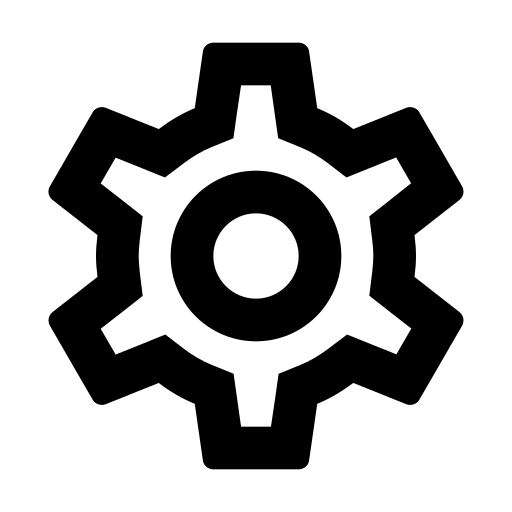
\includegraphics[width=3.5mm]{assets/google_icon_settings.png}
		\end{minipage}
	}
	\hspace{.8cm}
	\begin{minipage}{.24\textwidth}
		\Lirsting[float=H, fancyvrb={frame=none, fontsize=\footnotesize}, ranges={4-20}]{listings/simple_vm.s}
	\end{minipage}
	\Larrow{
		\begin{minipage}{.4cm}
			VM
		\end{minipage}
		\begin{minipage}{5mm}
			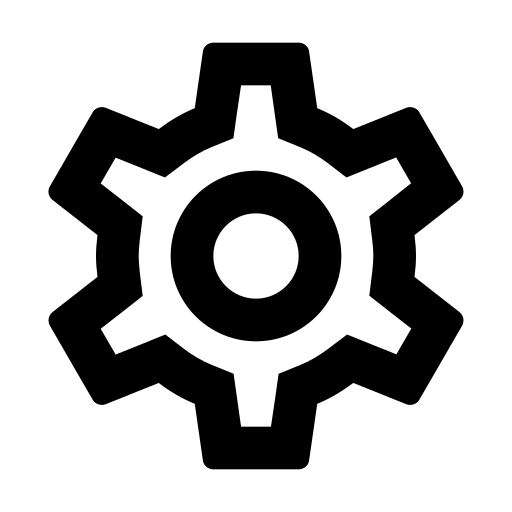
\includegraphics[width=3.5mm]{assets/google_icon_settings.png}
		\end{minipage}
	}
	\hspace{.1cm}
	\begin{minipage}{.13\textwidth}
		\centering
		{\large Exit code: 5}
	\end{minipage}
	\hfill

	\begin{itemize}
		\item Python, usw.
		\item Umwandlung in ein anderes Format
		\item[\Rightarrow] Anschliessende Ausführung des Programmes
	\end{itemize}
\end{frame}

\begin{frame}{Die rush VM}
	\pdfpcnote{
		@Mik \\
		\\
		- Diese Konzepte wurden nun auch auf die rush VM uebertragen \\
		\\
		--- \\
		\\
		- 1 Ausfuehrung vorher uebersetzter Programme\\
		- 2 **eine selbst entwickelte Architektur**, die das Ziel des Compilers darstellt \\
		- **stackbasiertes Design**, **hoher Abstaktionsgrad**
	}
	\begin{itemize}
		\item<1-> Führt ein zuvor übersetztes Programm aus
		\item<2-> Besitzt eine selbst entwickelte Architektur
			\begin{itemize}
				\item Stackbasiertes Design
				\item Hoher Abstaktionsgrad
			\end{itemize}
	\end{itemize}
\end{frame}

\begin{frame}{Felder der VM}
	\pdfpcnote{
		@Mik \\
		\\
		- Vgl. Tree-walking Interpreter: die VM hat 4 Felder \\
		\\
		--- \\
		\\
		1. **stack** fuer temporaere Werte \\
		2. **mem** und **mem-ptr** zur Speicherung von Variablen \\
		3. **call-stack** (also Aufrufstapel): verwaltet mehrere **Befehlszaehler** und **Funktionszaehler** \\
	}
	\begin{description}
		\item<1->[stack] Für temporäre Werte
		\item<2->[mem] Für Variablen
		\item<2->[mem\_ptr] Für Speicherverwaltung
		\item<3->[call\_stack] Aufrufstapel (\emph{Befehlsähler} und \emph{Funktionszähler})
	\end{description}
\end{frame}

\begin{frame}{Struktur der Programme der rush VM}
	\pdfpcnote{
		@Mik \\
		\\
		- 1 Die Programme der VM sind in Funktionen aufgeteilt \\
		- keinen Namen aber numerische Identifizierung \\
		- Jede Funktion enthaehlt mehrere Anweisungen \\
		- 2 Als Beispiel betrachten wir die Anweisung **call 2** \\
		- Der Befehlscode, also **call** \\
		- Und ein optionaler Operand, hier die **2** \\
		- 3 gerade einmal ca. 30 verschiedene Befehlscodes \\
	}
	\begin{itemize}
		\item<1-> Unterteilung in Funktionen
			\begin{itemize}
				\item Ohne Namen
				\item Numerische Identifizierung
				\item Enthält mehrere Anweisungen
			\end{itemize}
		\item<2-> Struktur der Anweisungen: \enquote{\LirstInline{asm}{call 2}}
			\begin{itemize}
				\item<2-> Befehlscode (\texttt{call})
				\item<2-> Optionaler Operand (\texttt{2})
			\end{itemize}
		\item<3-> ca. 30 verschiedene Befehlscodes
	\end{itemize}
\end{frame}

\begin{frame}{Demonstration: Ein-/Ausgabe}
	\pdfpcnote{
		@Mik \\
		\\
		- verschiedene Funktionen erkennbar (**Pointer**) \\
		\\
		--- \\
		\\
		- **call 2** wird an 2 Stellen verwendet: (7 und 29) \\
		- Wichtig ist: beim Abarbeiten der Anweisung springt die VM nur zur Anweisung in Zeile 10\\
		- Das heisst: es ist keine erneute Baumtraversierung notwendig \\
	}
	\begin{minipage}{0.5\textwidth}
		\Lirsting[float=H, fancyvrb={frame=none, fontsize=\small}]{deps/paper/listings/fib.rush}
		\centering
		\Larrow{Ausgabe}
	\end{minipage}
	\hfill
	\begin{minipage}{0.35\textwidth}
		\Lirsting[float=H, fancyvrb={frame=none, fontsize=\footnotesize}, ranges={1-20,26-32}]{listings/vm_fib.s}
	\end{minipage}
\end{frame}

\begin{frame}{Demonstration: Laufzeitverhalten}
	\pdfpcnote{
		@Mik \\
		\\
		- Nun betrachten Wir, wie die VM dieses Programm ausfuehrt \\
		- Man erkennt den Compiler nicht \\
		\\
		--- \\
		\\
		- Jeder Schritt: Abarbeitung einer Anweisung \\
		- Informationen: Felder der VM (**Stack oder die gespeicherten Variablen**) \\
	}
	\begin{figure}[H]
		\href{run:assets/01_rush_presentation_vm.mp4}{
			\movie{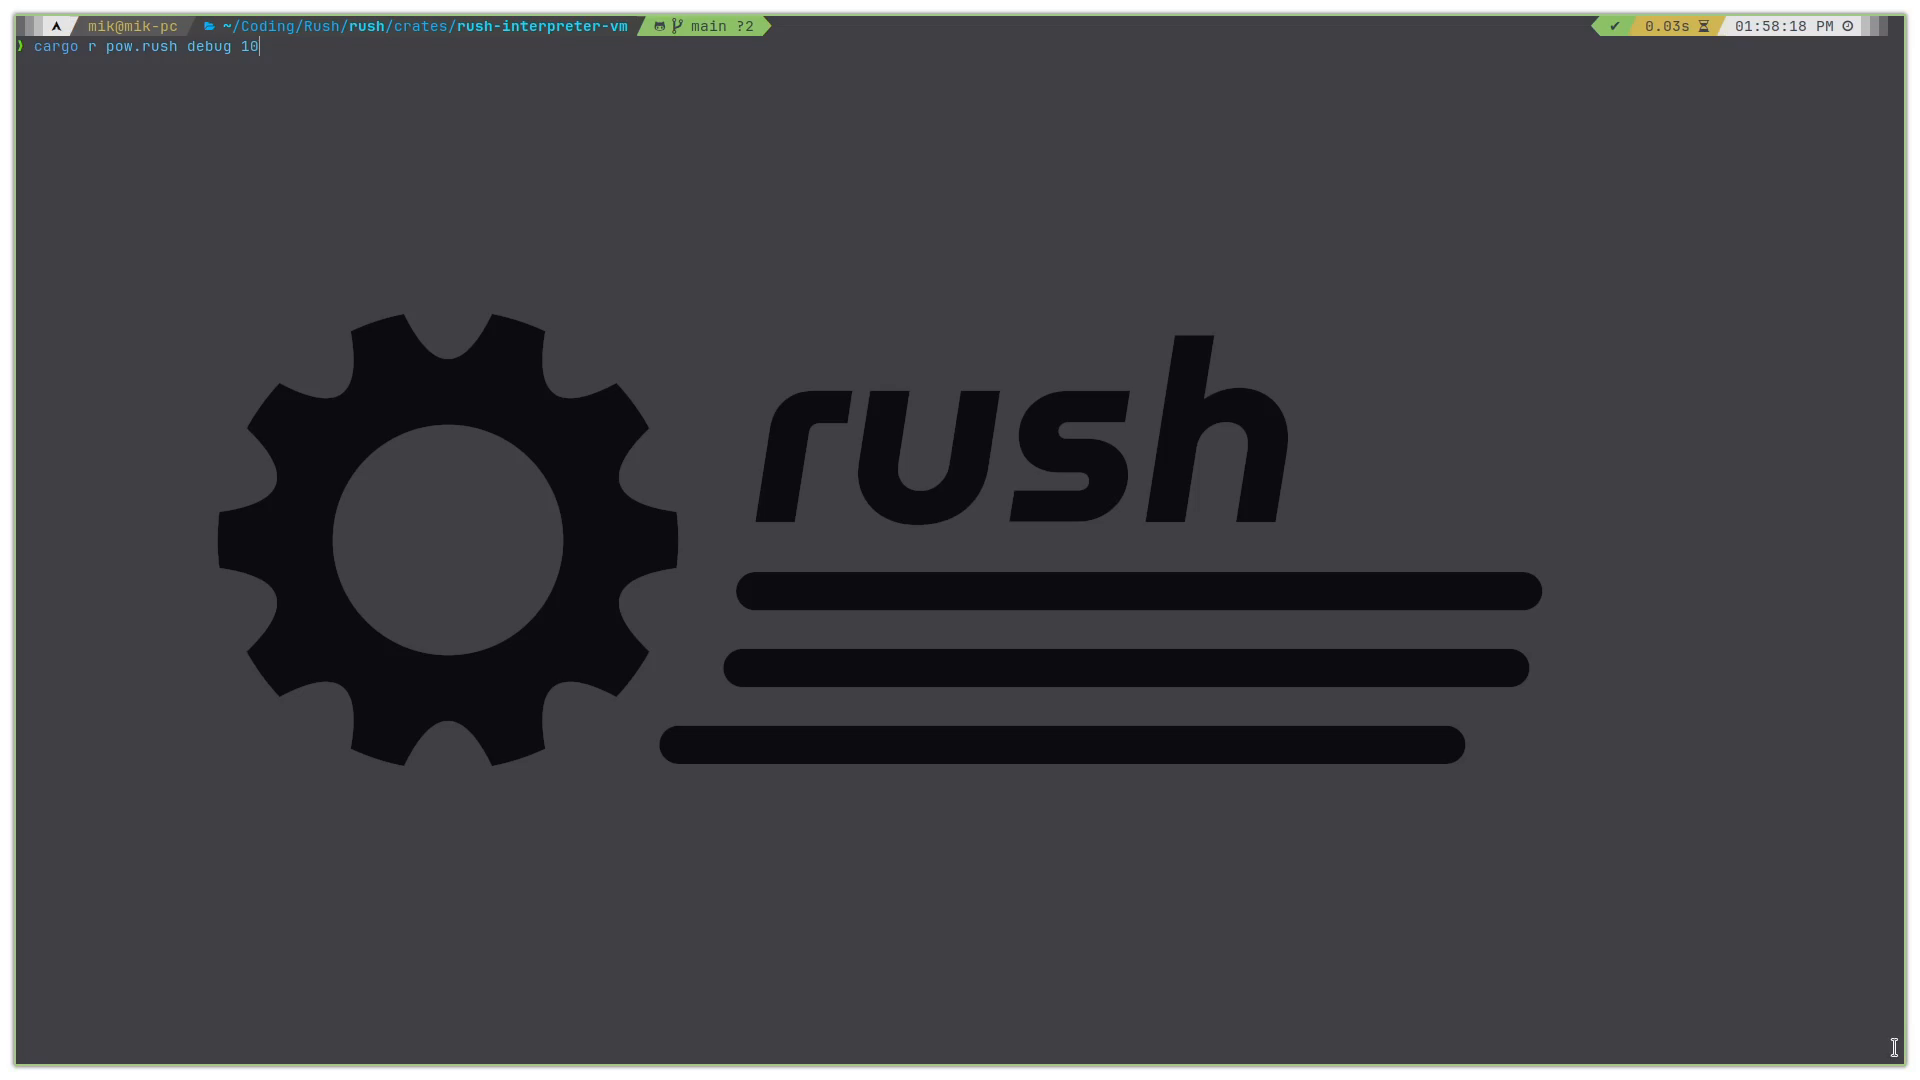
\includegraphics[width=.95\textwidth]{assets/01_rush_presentation_vm.png}}{assets/01_rush_presentation_vm.mkv}
		}
	\end{figure}
\end{frame}

\begin{frame}{VM: Fazit}
	\pdfpcnote{
		@Mik \\
		\\
		1. Durch  den Aufbau: die VM kann Programme ca. **2.7** mal schneller ausfuehren \\
		2. Implementierung vom Compiler hat sich als einfach herausgestellt \\
		- Stack-basierte Architektur \\
		- hoher Abstraktionsgrad der Architektur \\
		- gleichzeitige Entwicklung der VM und ihres Compilers \\
	}
	\begin{itemize}
		\item<1-> Ca. 2,7 mal schneller als der Tree-walking Interpreter
		\item<2-> Einfache Implementierung des Compilers
			\begin{itemize}
				\item<2-> Stack-basierte Architektur
				\item<2-> Hoher Abstraktionsgrad
				\item<2-> Gleichzeitige Entwicklung von VM und Compiler (\cemph{Feedbackschleife})
			\end{itemize}
	\end{itemize}
\end{frame}
